%%%%%%%%%%%%%%%%%%%%%%%%%%%%%%%%%%%%%%%%%%%%%%%%%%%%%%%%%%%%%%%%%%%%%%%%%%%%%%%%
% Limit_Setting.tex: Limit Setting
%%%%%%%%%%%%%%%%%%%%%%%%%%%%%%%%%%%%%%%%%%%%%%%%%%%%%%%%%%%%%%%%%%%%%%%%%%%%%%%%
\chapter{Limit  Setting and Interpretation}
\label{Limit_Setting_and_Interpretation_Chapter}
%%%%%%%%%%%%%%%%%%%%%%%%%%%%%%%%%%%%%%%%%%%%%%%%%%%%%%%%%%%%%%%%%

%%%%%%%%%%%%%%%%%%%%%%%%%%%%%%%%%%%%%%%%%%%%%%%%%%%%%%%%%%%%%%%%%%%%%%%%%%%%%%%%
\section{Exclusion Limit Setting}
%%%%%%%%%%%%%%%%%%%%%%%%%%%%%%%%%%%%%%%%%%%%%%%%%%%%%%%%%%%%%%%%%%%%%%%%%%%%%%%%
Since we did not find any excess of events over the expected SM background prediction we compute \textit{exclusion limits} based on our findings. In a search and discovery experiment, the exclusion limit is either an "upper" or a "lower" limit which is set on some \textit{Parameter Of Interest}~(POI) of a model, like the signal-strength modifier, $\mu$, which is directly related to the production cross-section of a new particle predicted to exist by the model. An exclusion limit on $\mu$ can be easily translated into exclusion limits on the mass and lifetime of the new particle allowing us to make following quantitative statements: 
\begin{itemize}
\item a Long-Lived Neutral Particle, if it exists, is produced with a cross-section below a certain threshold with this probability and the certain threshold is an \textbf{upper} limit on the Long-Lived Neutral Particle's production cross-section.
\item a Long-Lived Neutral Particle decay, if it happens, takes place with a mean lifetime larger than a certain threshold with this probability and the threshold is a \textbf{lower} limit on the Long-Lived Neutral Particle's mean lifetime.
\end{itemize}
Other equally important parameters like the uncertainties of the experiment, detector inefficiencies and luminosity  measurements which can impact the exclusions limits but are not the parameters under investigation by the analysis are called \textit{nuisance parameters}, usually denoted as $\mathbb{\theta}$. Nuisance parameters are used to introduce uncertainties in the computation of the exclusion limits.

%%%%%%%%%%%%%%%%%%%%%%%%%%%%%%%%%%%%%%%%%%%%%%%%%%%%%%%%%%%%%%%%%%%%%%%%%%%%%%%%%%%%%%%%%%%%%%%%%%%%%%%%
\subsection{$CL_{S}$ Method to Determine Exclusion Limits}
The $CL_{S}$ method is a statistical procedure used in a search and discovery experiment for evaluating exclusion limits and making constrains on the possible range of values of the fundamental parameters of a model which attempts to describe the observation or data from the experiment \cite{CLS}. The goal of the method is to constraint the value of the POI, $\mu$, and this is obtained from the ratio of the probabilities or $p$-values of the confidence interval derived from the signal plus background model or hypothesis to the background-only hypothesis. This ratio which is the $CL_{S}$ is defined as: 
\begin{equation}
CL_{S}  \equiv  \frac{CL_{s+b}}{CL_{b}} \equiv \frac{p_{s+b}}{1 - p_{b}}
\end{equation}
where $CL_{b}$ and $CL_{s+b}$ are the  probabilities of the confidence intervals derived from the background-only and signal plus background~($s+b$) hypothesis, respectively, and $p_{s+b}$ and $p_{b}$ are the $p$-values of $s+b$ and $b$-only hypothesis, respectively. 
The $CL_{S}$ is computed for different values of $\mu$ with each value signifying the level of signal contribution required to describe the observation. A set of values of $\mu$ in an experimentally defined region in the phase-space is excluded if the corresponding evaluated value of the $CL_{S}$ is below $0.05$ and this automatically corresponds to 95\% Confidence Level~(CL) in the excluded region of the parameter.
\newline
The $CL_{S}$ is the most favorable method compared to the $CL_{s+b}$ for evaluating the exclusion limits. This is because in some cases using the $CL_{s+b}$ produces limits where the background-only hypothesis is also excluded or the limit on the signal is negative~(large background and small observed number of events) and such limits are difficult to interpret. Thus with the $CL_{S}$ we are always guaranteed to produce non-negative limits. In other words, by \textit{normalizing} the $CL_{s+b}$~(dividing the $CL_{s+b}$ with the $CL_{b}$) we avoid producing erroneous limits like in the scenario where when the background rate, $b$, is small the evaluated interval using $CL_{S}$ still covers the true value unlike using the $CL_{s+b}$ procedure where when $b$ is small the procedure is more likely to produce an error \ie evaluates an interval which does not cover the true value \cite{LIM}. 
\newline
Theoretical, systematic and statistical uncertainties are taken into account in the $CL_{S}$ method through the use of nuisance parameters.

\subsection{Uncertainty Studies}
We have required in our event selection that the photon \pt be greater than 80\GeVc, the jet \pt be greater than 35\GeVc and the missing transverse energy be greater than 60\GeV. The same selection requirements applied to our MC signal event sample should guarantee a good event selection efficiency estimate. Any difference in the photon \pt, jet \pt and missing transverse energy between MC and data will be a source of systematic uncertainty on the efficiency of selecting signal events. These uncertainties can come from quantities like jet energy scale~(JES), jet energy resolution~(JER), electron-photon energy scale, instrumentation related and energy deposits not clustered during missing transverse energy reconstruction, photon arrival time bias and ECAL time resolution. 
\newline
Table \ref{tab:SYST} presents some of the sources of uncertainties considered in this analysis. The uncertainty values displayed are computed by varying by $1\sigma$ deviation of the nominal value of the given quantity, like JES, while keeping the values of the other uncertainty sources fixed and counting the number of events passing our event selection requirements. ECAL timing bias which has to do with the absolute reference time~(0\ns) of the ECAL time is the source of our largest uncertainty and since the photon arrival time is measured with respect to this reference time the ECAL time uncertainty has the largest impact on our analysis as our analysis is based on counting the number of events with photon ECAL time above $3$\ns. The next largest uncertainties are from energy deposits missed by the clustering algorithm. This affects the photon energy scale, missing transverse energy scale, jet energy scale and resolution.
The uncertainty on the photon energy scale in the barrel was estimated to be 4.0\%  which is based on measuring the photon energy of events with $Z\rightarrow \mu\mu\gamma$ decay where the muon radiates a photon in a process known as the final-state radiation~(FSR) \cite{PES}.  
\newline
The uncertainty on the \MET resolution uses a conservative estimate from \MET measurements in QCD events \cite{JES,METRES} where the \MET uncertainty is calculated using the fraction of events passing an event selection based on \MET for different \MET thresholds. 
\newline
The uncertainty on the ECAL time resolution was obtained by comparing the mean time of photons of events from $\gamma +$jet MC sample to events from data with photon ECAL time, $|t_{\gamma}| < 2$~ns. The difference is found to be of the order of 200\ps per event. 
\newline
Meanwhile, the systematic uncertainty on luminosity measurement has the recommended value of $2.2$\% provided by CMS and LHC luminosity measurements while the uncertainty from the measurement of the Parton Density Functions~(PDF) is evaluated using the re-weighting technique which uses the Master Equation of CTEQ65 model set described in \cite{PDF}.
\newline
The systematic uncertainties do not impact our results in a significant way since we use a data-driven method for estimating our background.
\newline
The statistical uncertainty in the \textsf{ABCD} background estimation method is our largest source of uncertainty in this analysis and we estimate it to vary upward by 223\% and downward by 51\%. This large background statistical uncertainty is because of the very low event yields. Our final result is affected by the signal selection efficiency only despite the large background estimation uncertainty. These signal selection uncertainties are used as nuissance parameters in the calculation of the upper limit on the observed signal cross-section~($\sigma_{UL}$).

\vspace{5mm}
\begin{minipage}{0.90\linewidth} 
\begin{center}
%\begin{table}[ht]
%\renewcommand\arraystretch{1.2}
\begin{tabular}{c c}
\toprule
\hline
\bfseries{Source} & \bfseries {Uncertainty(\%)}\\
\hline
\toprule
\texttt{ECAL absolute time }~(0.0~ns) & $<10.0$\% \\
\texttt{ECAL time resolution}~(0.5~ns) & $<5.0$\% \\
\texttt{Unclustered energy deposits} & $<9.0$\% \\
\texttt{Photon energy scale}  & $< 4.0$\% \\
\texttt{Jet energy scale}~(JES)  & $< 9.0$\% \\
\texttt{Jet energy resolution}~(JER) &$ <9.0$\% \\
\texttt{\MET resolution} & $ <2.8$\%  \\
\texttt{PDF uncertainty} & $< 1.70$\% \\
\hline
\toprule
\texttt{Background estimation uncertainty} &$51.0$\% to 223\% \\
\hline 
\texttt{Luminosity}~(4.5\%) & $< 2.2$\% \\
\hline
\bottomrule
\end{tabular}
\captionof{table}{Summary of systematic uncertainties for signal efficiency and background estimation in this analysis and applied to our final results.}
\label{tab:SYST}
%\end{table}
\end{center}
\end{minipage}
\clearpage

%%%%%%%%%%%%%%%%%%%%%%%%%%%%%%%%%%%%%%%%%%%%%%%%%%%%%%%%%%%%%%%%%%%%%%%%%%%%%%%%%%%%%%%%%%%%%%%%%%%%%%%%
\subsection{The \textsc{HiggsCombine} Tool for Evaluating Upper Limits}
CMS has developed a statistical software package which implements the $CL_{S}$ method for hypothesis testing and evaluating confidence limits called \textsc{HiggsCombine} \cite{LIMITS}. The  \textsc{HiggsCombine} tool provides access to a variety of robust statistical methods with optimized performance for computing limits and takes as input the expected number of events or a histogram of the signal, the estimated background, the observed number of events from data and the uncertainties and produces an upper limit in the signal-strength modifier, $\mu$, which is translated to the production cross-section of a given physics process. In addition to the numerous computing and optimization advantages, the \textsc{HiggsCombine} tool allows for the possibility of using several different statistical inference methods like Frequentist, Bayesian, Analytical and Hybrid methods to compute the upper limits. Through this way we  are able to make comparisons and perform simple checks for any inconsistency. In this analysis we used the prescribed HybridNew~(a hybrid of Frequentist and Bayesian methods) method to evaluate the observed  limits. We describe in detail in the next subsections how the statistical hypothesis testing is formulated and upper limits are derived.

\subsubsection{Statistical Test Formalism}
The objective of a statistical test is to set upper limits on the cross-sections derived from a signal plus background hypothesis which in our case is the SPS8 benchmark GMSB model. The region of the phase-space of the cross-section defined by the POI, $\mu$, of the SPS8  benchmark GMSB model which fails the goodness-of-fit test to the observed data which is the result of our search experiment  is excluded. The statistical formalism to perform such a test goes in the following way. 
\newline
Since our search experiment is an event counting experiment, we construct a histogram in the photon ECAL time of the number of events, $\mathbf{M}$, passing our final event selection and acceptance. Suppose the number of events in each bin of the histogram is $n_{i}$ with $i = 1, \cdots, N$, where $N$ is the number of bins of the histogram. Since we only observed a single event filling just one bin this means $N = 1$. The expected number of events in the $i^{th}$ bin given as:
$ E[n_{i}] = \mu s_{i} + b_{i}$, is the sum of events from all known physics processes which is a combination of events due to the Standard Model which we  call background events, $b_{i}$, and events due to the  SPS8 benchmark GMSB model which we call signal events, $s_{i}$. The signal-strength modifier, $\mu$, being the POI relates the expected cross-section~($\sigma_{th}$) as predicted by the SPS8  benchmark GMSB model to the actual observed cross-section~($\sigma^{Obs}$) as
\begin{equation}
\mu = \frac{\sigma^{Obs}}{\sigma_{th}}.
\end{equation}
When $\mu = 0$ it means the  SPS8  benchmark GMSB model contributes nothing to the number of events in each bin and gives an opportunity to test the Standard Model background-only hypothesis.
\newline
When $\mu=1$ it means the SPS8  benchmark GMSB theory contributed to the number of events in each bin and gives an opportunity to tests the signal plus background hypothesis. 
\newline
The other values for $\mu$ corresponds to different rates of contribution by the SPS8 benchmark GMSB model.
\par 
In order to measure the compatibility of a given hypothesis to the observed data we define a joint probability density function called the \textit{likelihood}. The cross-section of an interesting event like a new particle is very low compared to the total cross-section of any scattering event happening, as a result, the likelihood function, $\mathcal{L}$, is the product of the Poisson probabilities for all the bins of the histogram:
\begin{equation}\label{eq:LL}
\mathcal{L}\left( \mu, \mathbf{\theta} \right) = \prod^{N}_{i=1} \frac{{\left( \mu s_{i} + b_{i} \right)}^{n_{i}}}{n_{i}!} e^{-(\mu s_{i} + b_{i})} \cdot \mathcal{G}(\mathbf{\theta} ),
\end{equation}
where $\mathcal{G}(\mathbf{\theta})$ is a product of probability distributions of the \textit{nuisance parameters} through which the uncertainties which impact the limit on $\mu$ are introduced. This probability distributions can be different for different uncertainties ranging from Poisson, log-normal, Gaussian and Gamma distributions. In our evaluation of the exclusion limits in this analysis we introduced all the uncertainties presented in Table \ref{tab:SYST} as nuisance parameters with log-normal distributions.
In the $CL_{S}$ method the uncertainties are treated differently depending on the method used to perform the statistical inference. In the HybridNew method which is prescribed by both CMS and ATLAS experiments to compute upper limits  the uncertainties are treated according to the Frequentists methods by "marginalizing" the likelihood \ie integrating out all the nuisance parameters. 
%%%%%%%%%%%%%%%%%%%%%%%%%%%%%%%%%%%%%%%%%%%%%%%%%%%%%%%%%%%%%%%%%%%%%%%%%%%%%%%%%%%%%%%%%%%%%%%%%%%%%%%
\subsubsection{Test-Statistics and $p$-values} 
According to the Neyman-Pearson theorem the profile likelihood ratio gives the most powerful hypothesis test \cite{NPT}. Therefore using the marginalized likelihood function we define the \textit{profile likelihood} ratio~(for simplicity, instead of writing the explicit dependence of $\mathcal{L}$ on $n_{i}$ we write  $\mathcal{L}$ in terms of the parameters) as
\begin{equation}\label{eq:PLL}
\lambda(\mu) =  \frac{\mathcal{L}(\mu, \hat{\hat{\mathbf{\theta}}})}{\mathcal{L}(\hat{\mu}, \hat{\mathbf{\theta}} )}
\end{equation}
where $\hat{\hat{\mathbf{\theta}}}$ is the \textit{conditional maximum-likelihood estimator}~(CMLE) of $\mathbf{\theta}$ and it is the the value of $\mathbf{\theta}$ that maximizes $\mathcal{L}$ for a fixed value of $\mu$. $\hat{\hat{\mathbf{\theta}}}$ is a function of $\mu$.  $\mathcal{L}(\hat{\mu}, \hat{\mathbf{\theta}} )$ is the maximized (unconditional) likelihood function with $\hat{\mu}$ and $\hat{\mathbf{\theta}}$ being its \textit{maximum likelihood}~(ML) estimators for each Monte Carlo simulated toy experiment or real data. 
\newline
The nuisance parameter causes a broadening of the distribution of the profile likelihood ratio and this reflects the loss in sensitivity or loss of information about the parameter $\mu$ due to the uncertainties.% This broadening can be seen in a plot of the profile likelihood ratio as a function of $\mu$.
\newline
The expression for $\lambda(\mu)$ given in Equation \ref{eq:LL} suggest that $0 \leq \lambda(\mu) \leq 1$. When $\lambda(\mu)$ is close to 1 it means $\mu$ is compatible with data. Thus, in order to assess the agreement between the observed data with either the background-only or signal plus background hypothesis we define a quantity called the \textit{test-statistics}. The test-statistics is used to distinguish between two hypothesis based on the agreement of their predictions with data. Our choice of test-statistics is the \textit{profile log-likelihood ratio} given as
\begin{equation}
 q_{\mu} = -2\ln \lambda(\mu),
\end{equation}
with the compatibility between these hypothesis and data taking an even more simpler interpretation: higher values of the test-statistics indicates that the assumed level of the signal represented by the value of $\mu$ is incompatible with data compared to the background-only hypothesis. The level of incompatibility is quantified using a probability or $p$-value which is derived from the Probability Density Distribution~(PDD) of the test-statistics, $f(q_{\mu}|\mu)$. The analytic evaluation of $f(q_{\mu}|\mu)$ is generally very difficult so in practice $f(q_{\mu}|\mu)$ is approximated by evaluating $q_{\mu}$ for a large number of simulated toy experiments with the simulated data obtained by Monte-Carlo generating Poissonian random numbers with the expected number of events according to the model prediction for a given value of $\mu$. By repeating this process for different values of $\mu$ we sample the distribution of $f(q_{\mu}|\mu)$.
%%\ie for a given value of the POI, $ \mu^{\prime}$, $f(q_{\mu}|\mu^{\prime})$ is estimated from a sample of simulated toy experiments  generated through Monte Carlo with an assumption that $\mu = \mu^{\prime}$.
\newline
For the signal plus background hypothesis, the $p$-value for the signal plus background hypothesis being compatible with the data is evaluated as 
\begin{equation}
 CL^{(\mu)}_{s+b} = p_{s+b} = \int^{\infty}_{q^{obs}_{\mu}} f(q_{\mu}|\mu) dq_{\mu},
\end{equation}
where $q^{obs}_{\mu}$ is the value of the test-statistics~($q_{\mu}$) from the real data. Large values of $ CL^{(\mu)}_{s+b}$ suggests that chances are high that the observation is compatible with the prediction of the signal plus background hypothesis.
\newline
For the background-only hypothesis, the test-statistics  is defined with $\mu = 0$ as
%\begin{equation}\label{eq:HNULL}
\[\label{eq:HNULL}
 q_{\mu} = \left\lbrace  
  \begin{array}{ll}
 -2\ln \lambda(0), & \hat{\mu} \geq 0 \\
   0,              & \hat{\mu} \leq 0
  \end{array}
  \right.
\]
where $\lambda(0)$ is the profile log-likelihood ratio with $\mu = 0$ defined in Equation \ref{eq:PLL}.
The probability or $p$-value for the background-only~($\mu = 0$) hypothesis being compatible with the data is evaluated as
\begin{equation}\label{eq:HALT}
 CL^{(\mu)}_{b} = 1 - p_{b} = \int^{\infty}_{q^{obs}_{\mu}} f(q_{\mu}|0) dq_{\mu},
\end{equation}
where $f(q_{\mu}|0)$ is the PDD of the test-statistics, $q_{\mu = 0}$, under the background-only~($\mu = 0$) hypothesis and is also approximated using simulated toy experiments. The $CL_{b}$ probability measures the disagreement of the data and the prediction from the background-only hypothesis.
%%%%%%%%%%%%%%%%%%%%%%%%%%%%%%%%%%%%%%%%%%%%%%%%%%%%%%%%%%%%%%%%%%%%%%%%%%%%%%%%%%%%%%%%%%%%%%%%%%%%%%%
\clearpage
\subsubsection{The $CL_{S}$ value and exclusion limits} 
Using Equations \ref{eq:HNULL} and \ref{eq:HALT} the probability, $ CL^{(\mu)}_{S}$, given as
\begin{equation}
CL^{(\mu)}_{S} \equiv \frac{CL^{(\mu)}_{s+b} }{ CL^{(\mu)}_{b}},
\end{equation}
measures how well we can statistically distinguish the signal plus background from the background only hypothesis looking at the data. Small values of the $CL^{(\mu)}_{S}$ indicates that the data strongly favors the background-only hypothesis over the signal plus background hypothesis.
\newline
The $CL^{(\mu)}_{S}$ is used to obtain an exclusion limit on the POI, $\mu$, with some confidence level commonly referred to as $CL^{(\mu)}_{S}$ Confidence Levels~(CL). By increasing the value of $\mu$~(increasing the contribution of the signal) the $CL^{(\mu)}_{S}$ decreases down to a certain threshold value. The threshold value for which $CL^{(\mu^{UL})}_{S} = \alpha$ is the \textbf{upper limit} for $\mu$ at the desired $1-\alpha$\% CL. At 95\% $CL_{S}$ confidence level, $\alpha = 0.05$. 
\newline
From the observed data, the observed test-statistics, $q^{obs}_{\mu}$, gives the \textbf{observed} upper limit and the interpretation of the limit is such a prediction by the signal plus background hypothesis corresponding to $\mu > \mu_{obs}^{UL}$ is excluded at a 95\% CL and $\mu_{obs}^{UL}$ is the upper limit of $\mu$.
\newline
From the simulated toy Monte Carlo data, the median of the test-statistics obtained from the background-only hypothesis with $\mu = 0$ gives the \textbf{expected} exclusion limit~($\mu_{med}^{UL}$) of the SPS8 benchmark GMSB model. This expected limit is used to quantify the sensitivity of the search experiment.
\newline
In addition to the expected limit we are also interested in quantifying the range of possible statistical deviations from the median \ie how much the expected exclusion limit can statistically fluctuate upward or downward due to statistical uncertainties and so we evaluate the 68\%~($+1\sigma$), 16\%~($-1\sigma$), 98\%~($+ 2\sigma$) and 2.5\%~($-2\sigma$) errors on the median. The exclusion limits obtained with the $CL_{S}$ method are presented in exclusion plot where the observed limits obtained from the experiment and the expected limits are displayed simultaneously. Figure \ref{fig:SPS8_Ctau_Ulimit} shows an exclusion plot where the dashed red line represent the expected limit while the \textbf{green} and \textbf{yellow} bands represents the $\pm1\sigma$ and $\pm2\sigma$ errors on the expected limit, respectively. These deviations from the median expected limit allows us to assess the exclusion potential of the search experiment. The \textbf{observed} limit is indicated by the solid black line.
%%%%%%%%%%%%%%%%%%%%%%%%%%%%%%%%%%%%%%%%%%%%%%%%%%%%%%%%%%%%%%%%%%%%%%%%%%%%%%%%%%%%%%%%%%%%%%%%%%%%%%%%%%%%%%%%%
%%#######################################################################################################
%\clearpage
\section{Limit Interpretation in the SPS8 Benchmark GMSB Model}
%%%%%%%%%%%%%%%%%%%%%%%%%%%%%%%%%%%%%%%%%%%%%%%%%%%%%%%%%%%%%%%%%%%%%%%%%%%%%%%%%%%%%%%%%%%%%%%%%%%%%%
We set upper limits at 95\% $CL_{S}$ confidence level on the product of the production cross-section and branching ratio for the decay of the lightest neutralino~(\PSneutralinoOne) into a photon~(\Pphoton) and gravitino~($\tilde{G}$) as predicted by the SPS8 benchmark GMSB model. The exclusion limits are presented in an exclusion plot as a function of the mean lifetime, $\tau_{\PSneutralinoOne}$(\ns), and the mass of the lightest neutralino, $m_{\PSneutralinoOne}$(\GeVcc),  or equivalently the effective SUSY breaking scale, $\mathbf{\Lambda}$\TeV.
%%%%%%%%%%%%%%%%%%%%%%%%%%%%%%%%%%%%%%%%%%%%%%%%%%%%%%%%%%%%%%%%%%%%%%%%%%%%%%%%%%%%%%%%%%%%%%%%%%%%%%
\subsection{Cross-section Upper Limits}
The \textsc{HiggsCombine} tool gives us an upper limit on the number of events, $N_{UL}$, and knowing our signal event selection efficiency~($\varepsilon$) and acceptance~($A$) we can compute the upper limit on the cross-section as
\begin{equation}{\label{eq:SIGMAUPA}}
\sigma_{UL} = \frac{N_{UL}}{\varepsilon\times A\cdot \mathscr{L}},
\end{equation}
where $\mathscr{L}$ is the integrated luminosity~(19\fbinv).
%and we have used the relationship between the cross-section~($\sigma$) the number of events~($N$): $\sigma = \frac{N}{\varepsilon\times A \cdot \mathscr{L}}$.

\subsubsection{Signal Efficiency and Acceptance}
%%%%%%%%%%%%%%%%%%%%%%%%%%%%%%%%%%%%%%%%%%%%%%%%%%%%%%%%%%%%%%%%%
The plot in Figure \ref{fig:EffAcc} shows our signal event selection efficiency and acceptance for  events from signal MC samples for different mean lifetime or \textit{proper decay length}, $c\tau$, ranging from 500\mm~($\tau = 1.7\ns$) to 6000\mm~($\tau = 20.0\ns$) with the same lightest neutralino mass of 255\GeVcc or equivalently $\mathbf{\Lambda=180}$\TeV. 

\vspace{5mm}
\begin{minipage}{0.90\linewidth} 
\begin{center}
%\mbox{
%\includegraphics[width=0.49\textwidth,height=0.5\textwidth]
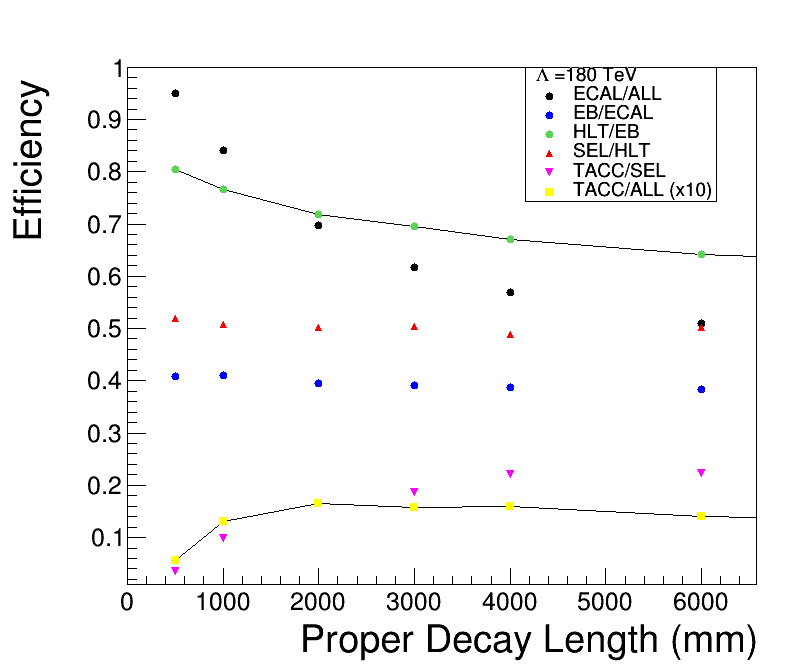
\includegraphics[height=0.65\textwidth, width=0.8\textwidth]{THESISPLOTS/Eff_180_ctau_2015.png}
%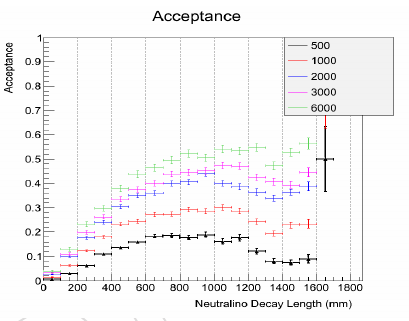
\includegraphics[height=0.5\textwidth, width=0.5\textwidth]{THESISPLOTS/SignalReconstructionAcceptance.png}}
\captionof{figure}{The efficiency for different mean decay length, $c\tau$~[\mm] with  $\mathbf{\Lambda}=180$\TeV. TACC/ALL~(yellow square markers) is the  Efficiency $\times$ Acceptance($t>3$\ns) \ie $\varepsilon \times A$, used in evaluating the exclusion limits. The TACC/ALL is magnified by factor $\times 10$ for display purpose. }
\label{fig:EffAcc}
\end{center}
\end{minipage}

\vspace{5mm}
The efficiency plot is described as follows: \textsc{ALL} means all the photons from the decay of the MC generated lightest neutralino, \textsc{ECAL} means the photons in barrel~(EB) and endcaps~(EE) inclusive, \textsc{EB} means only reconstructed photons in EB are selected, \textsc{HLT} means the photon triggered our HLT trigger, \textsc{SEL} means the events passed our event selection requirement and \textsc{TACC} means the event pass our event selection and the photon acceptance of $t>3.0\ns$. Each ratio defines an efficiency at a different event selection stage.
The important efficiency to focus on is the TACC/ALL defined as the ratio of the events passing our event selection with photon time, $t > 3$\ns in the barrel to all the events with photons from the decay of the generated lightest neutralino since this is the efficiency times acceptance~($\varepsilon \times A$) used in Equation \ref{eq:SIGMAUPA} to evaluate the exclusion limits on the cross-section. 
\newline
The efficiency time acceptance TACC/ALL is small~(less than 1\%) for smaller values of $c\tau = 500\mm$~($\tau = 1.7$\ns) since very few of the events from the lightest neutralino decay have photons with time, $t > 3$\ns despite many of the photons reaching ECAL as shown by the ECAL/ALL efficiency which is defined as the ratio of events with photons reaching ECAL to all events with photons from the decay of the generated lightest neutralino. This indicates that the efficiency without the 3.0\ns requirement is high for low $c\tau$ values.  The TACC/ALL begins to slowly rise with $c\tau$ up to $c\tau = 2000\mm$~($\tau = 6.7$\ns) where it has a maximum value of about 1.6\% and then begins to fall again~(less than 1\%) for large $c\tau$ values. The fall with large $c\tau$ values~($c\tau > 6000\mm$) is because most of the lightest neutralinos decay outside of the ECAL and are undetected. %%%%%%%%%%%%%%%%%%%%%%%%%%%%%%%%%%%%%%%%%%%%%%%%%%%%%%%%%%%%%%%%%%%%%%%%%%%%%%%%%%%%%%%%%%%%%%%%%%%%%%%
%%%% Upper Limits Described Theory cross-section prediction & Already excluded limits \ie where upper limts are lower than prediction & current exclusion limits
\par 
The predicted product of cross-section and branching ratio~($\sigma\times BR$) for the production and decay of the lightest neutralino according to the SPS8 benchmark GMSB model at Leading Order~(LO) interactions  for effective SUSY breaking scale, $\mathbf{\Lambda} = 180\TeV$ and is 0.015\pba shown as the blue line in Figure \ref{fig:SPS8_Ctau_Ulimit}. The theoretical cross-section falls with increasing values of $\mathbf{\Lambda} = 180\TeV$ as shown in Figure \ref{fig:MASS-limits}.
\newline
Prior to this search experiment, the upper limit set on the product of the lightest neutralino production cross-section and branching ratio decay to a photon and gravitino channel, $\PSneutralinoOne \rightarrow \gamma + \tilde{G}$, according to the SPS8 benchmark GMSB model at by CMS was $\sigma^{UP}_{\PSneutralinoOne} \times BR < 0.02\pba$, for lightest neutralino mass of 215\GeVcc or equivalently effective SUSY breaking scale of 154\TeV and $c\tau = 1\mm$ \cite{CMS}. From the results of this search experiment, using Equation \ref{eq:SIGMAUPA} we set an upper limit of $\sigma\times BR = 0.0125$\pba and the corresponding mean lifetime of the lightest neutralino, $\tau_{\PSneutralinoOne}$, to be either less than $3.2$\ns or larger than 19.87\ns for  $\mathbf{\Lambda} = 180\TeV$ or equivalently mass of lightest neutralino, $m_{\PSneutralinoOne} = 255\GeVcc$, shown in Figure \ref{fig:SPS8_Ctau_Ulimit}. For other lightest neutralino masses and mean lifetimes their corresponding cross-section upper limits can be read directly from Figure \ref{fig:SPS8_SIGMA-Ulimit} which indicates the region in  $\mathbf{\Lambda}$ and $\tau_{\PSneutralinoOne}$ where the ECAL sub-detector is most sensitive to the decay of \PSneutralinoOne or LLNPs to late photons. 
%%%%%%%%%%%%%%%%%%%%%%%%%%%%%%%%%%%%%%%%%%%%%%%%%%%%%%%%%%%%%%%%%%%%%%%%%%%%%%%%%%%%%%%%%%%%%%%%%%%%%%%%
\subsection{Mass and Lifetime Upper Limits}
Using the cross-section from theory~(shown as the blue line in Figure \ref{fig:SPS8_Ctau_Ulimit}, for example), the excluded region in the mean lifetime of the lightest neutralino according to the SPS8 benchmark GMSB model are the values of mean lifetime, $\tau$, for which the observed cross-section is below the theory cross-section, \ie a lower limit and an upper limit on $\tau$ is extracted for the corresponding points where the observed cross-section and the theory cross-section intersect.
An exclusion  upper limit on the mass or effective SUSY breaking scale, $\mathbf{\Lambda}$, is obtained from Figure \ref{fig:MASS-limits} at the point where the observed cross-section~(solid black line) intersects with the expected~(blue line) cross-section. 
\newline
The excluded lightest neutralino mass, $m_{\PSneutralinoOne}$, or effective SUSY breaking scale, $\mathbf{\Lambda}$, observed from the cross-section against lightest neutralino mass plot of Figure \ref{fig:MASS-limits} for $\tau = 6.7$\ns is up to  $m_{\PSneutralinoOne} = 300\GeVcc$ or  $\mathbf{\Lambda} = 220\TeV$, still in the context of the SPS8 benchmark GMSB model.
\newline
From the 2 dimensional plane define by $(\mathbf{\Lambda},\tau_{\PSneutralinoOne})$ of the exclusion limit shown in  Figure \ref{fig:SPS8_2D-Ulimit}, the excluded lightest neutralino mean lifetime, $\tau_{\PSneutralinoOne}$, is from $2.0$\ns to $45.0$\ns for low mass~($m_{\PSneutralinoOne} < 150\GeVcc$) lightest neutralino. This exclusion in mean lifetime shrinks as the mass of the lightest neutralino increases or effective SUSY breaking scale increases. This is because the production cross-section for the lightest neutralino decreases with increase in its mass or $\mathbf{\Lambda}$. 

\vspace{5mm}
\begin{minipage}{0.90\linewidth}
\begin{center}
%\mbox{
%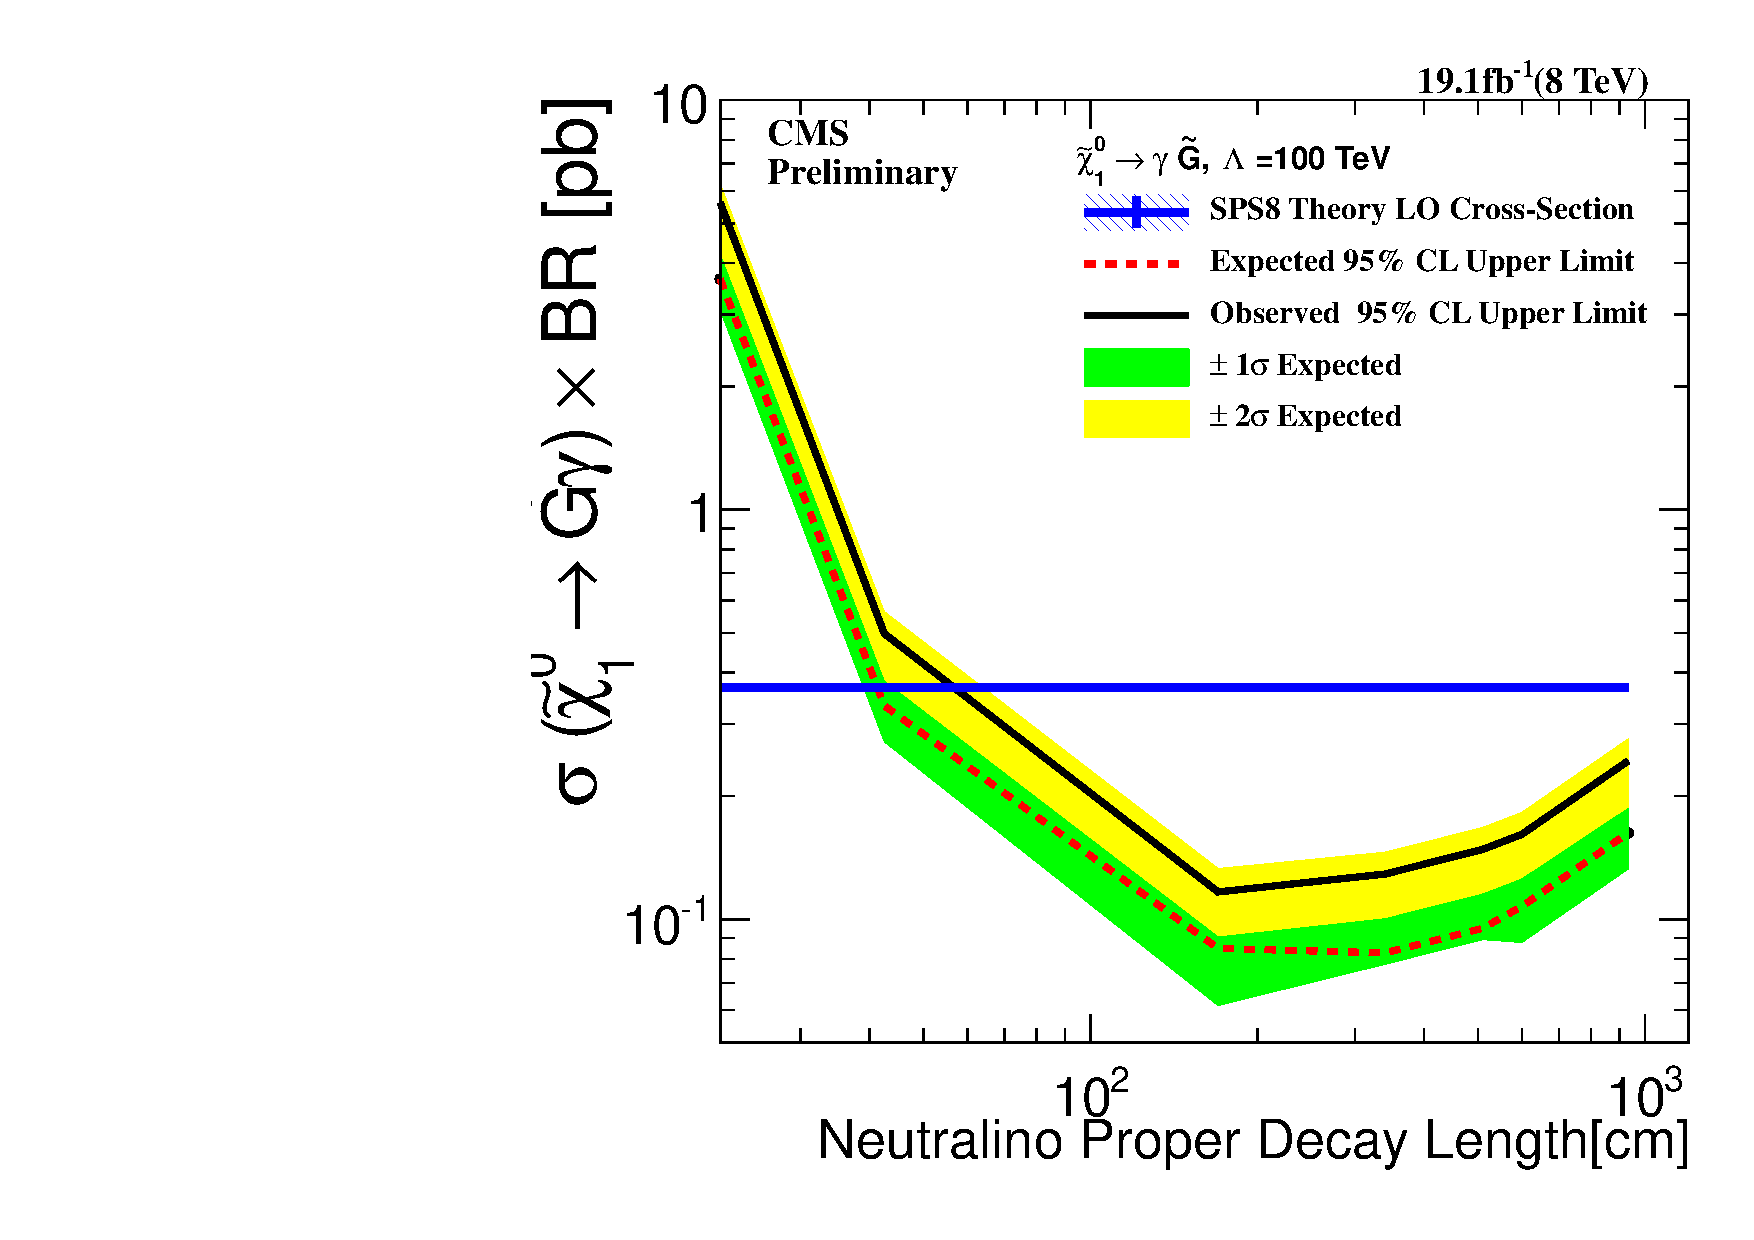
\includegraphics[height=0.65\textwidth, width=0.53\textwidth]{THESISPLOTS/100TeV_Neutralino_CrossSecTimesBR_Uplimit.pdf}
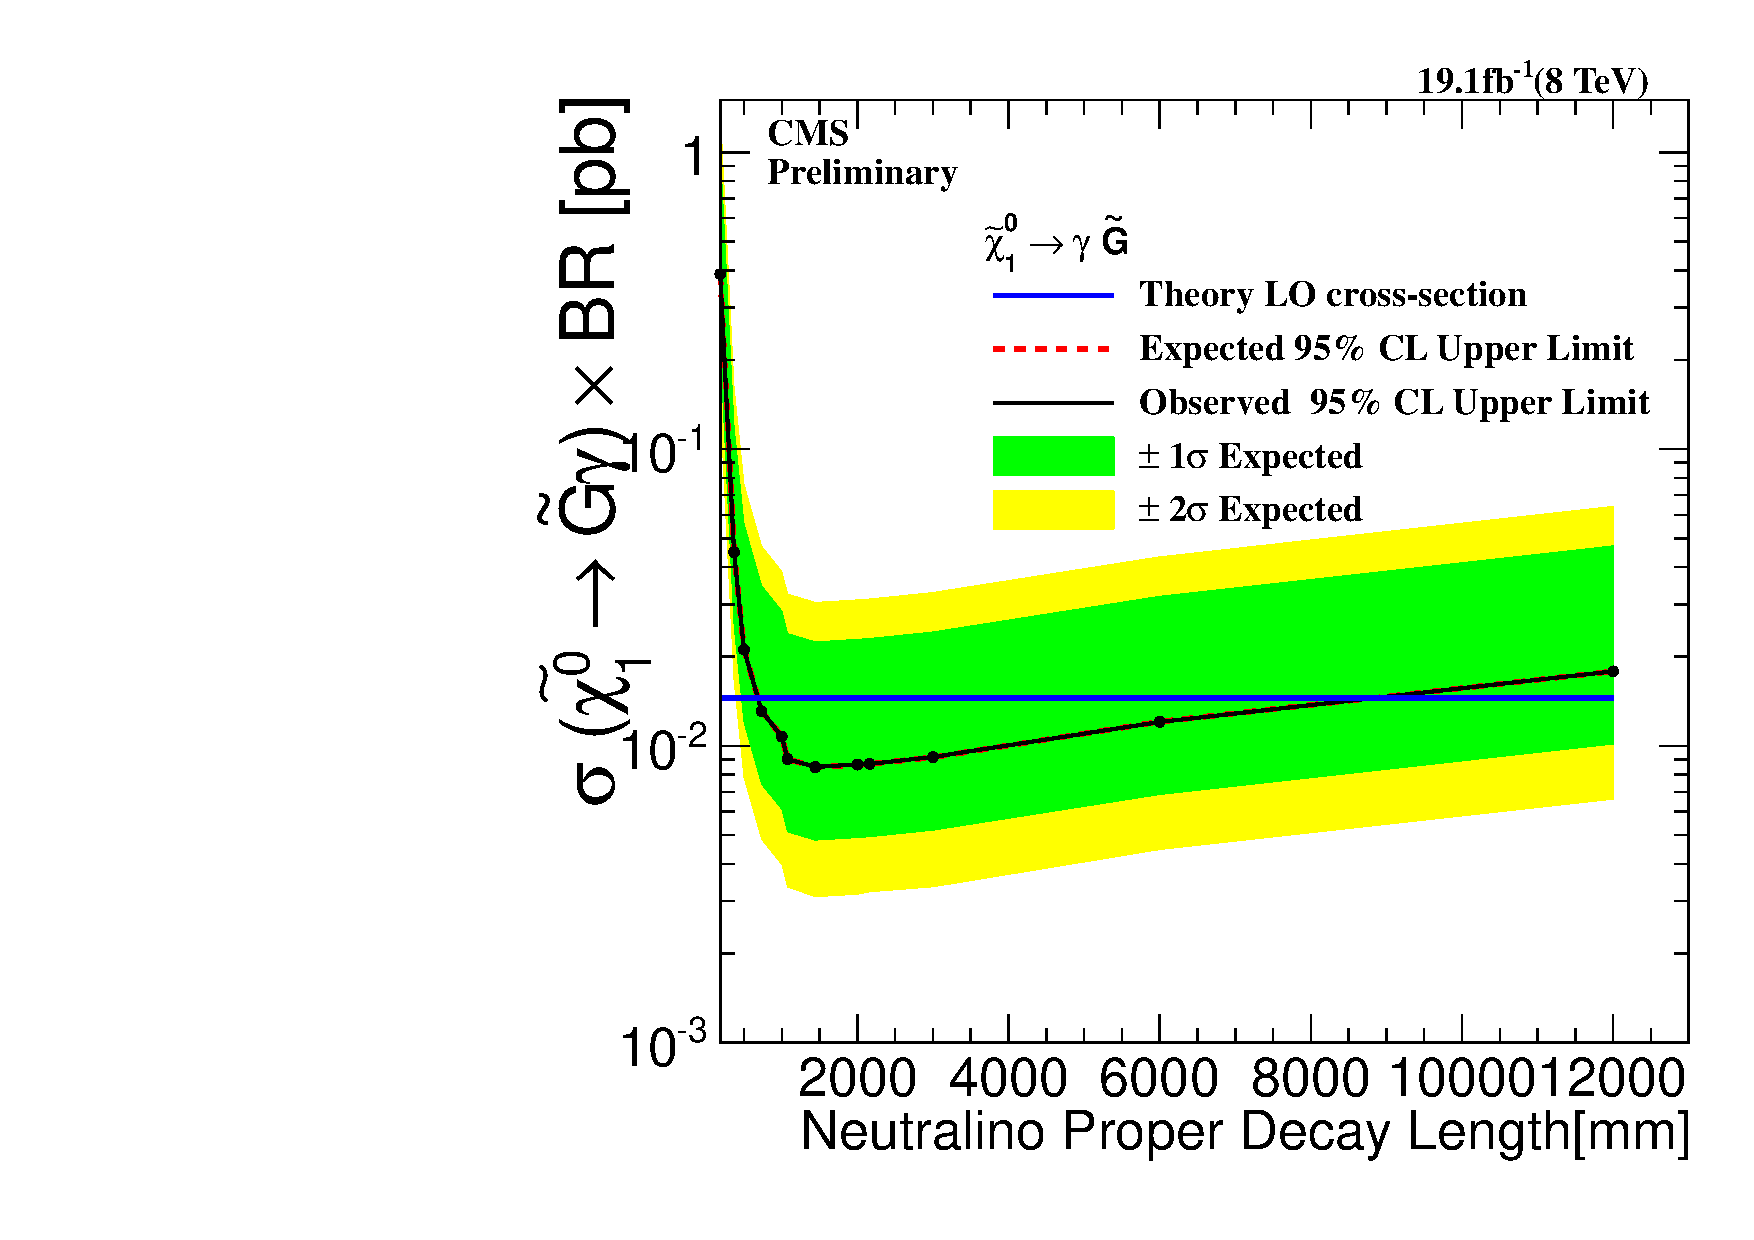
\includegraphics[height=0.8\textwidth, width=0.85\textwidth]{THESISPLOTS/Neutralino_CrossSecTimesBR_Uplimit.pdf} 
%}
\captionof{figure}{ 95\% $CL_{S}$ CL on the lightest neutralino production cross-section times branching ratio~($\sigma\times BR$) against mean lifetime[\ns] for $\mathbf{\Lambda = 180}$\TeV in the SPS8 benchmark GMSB model.}
\label{fig:SPS8_Ctau_Ulimit}
\end{center}
\end{minipage}
\vspace{5mm}

\vspace{5mm}
%\begin{figure}[!htb]
\begin{minipage}{0.90\linewidth}
%%\afterpage{ %
 %% \clearpage% Flush earlier floats (otherwise order might not be correct)
   %% \thispagestyle{empty}% empty page style (?)
%%\begin{landscape}% Landscape page
\begin{center}
%\mbox{
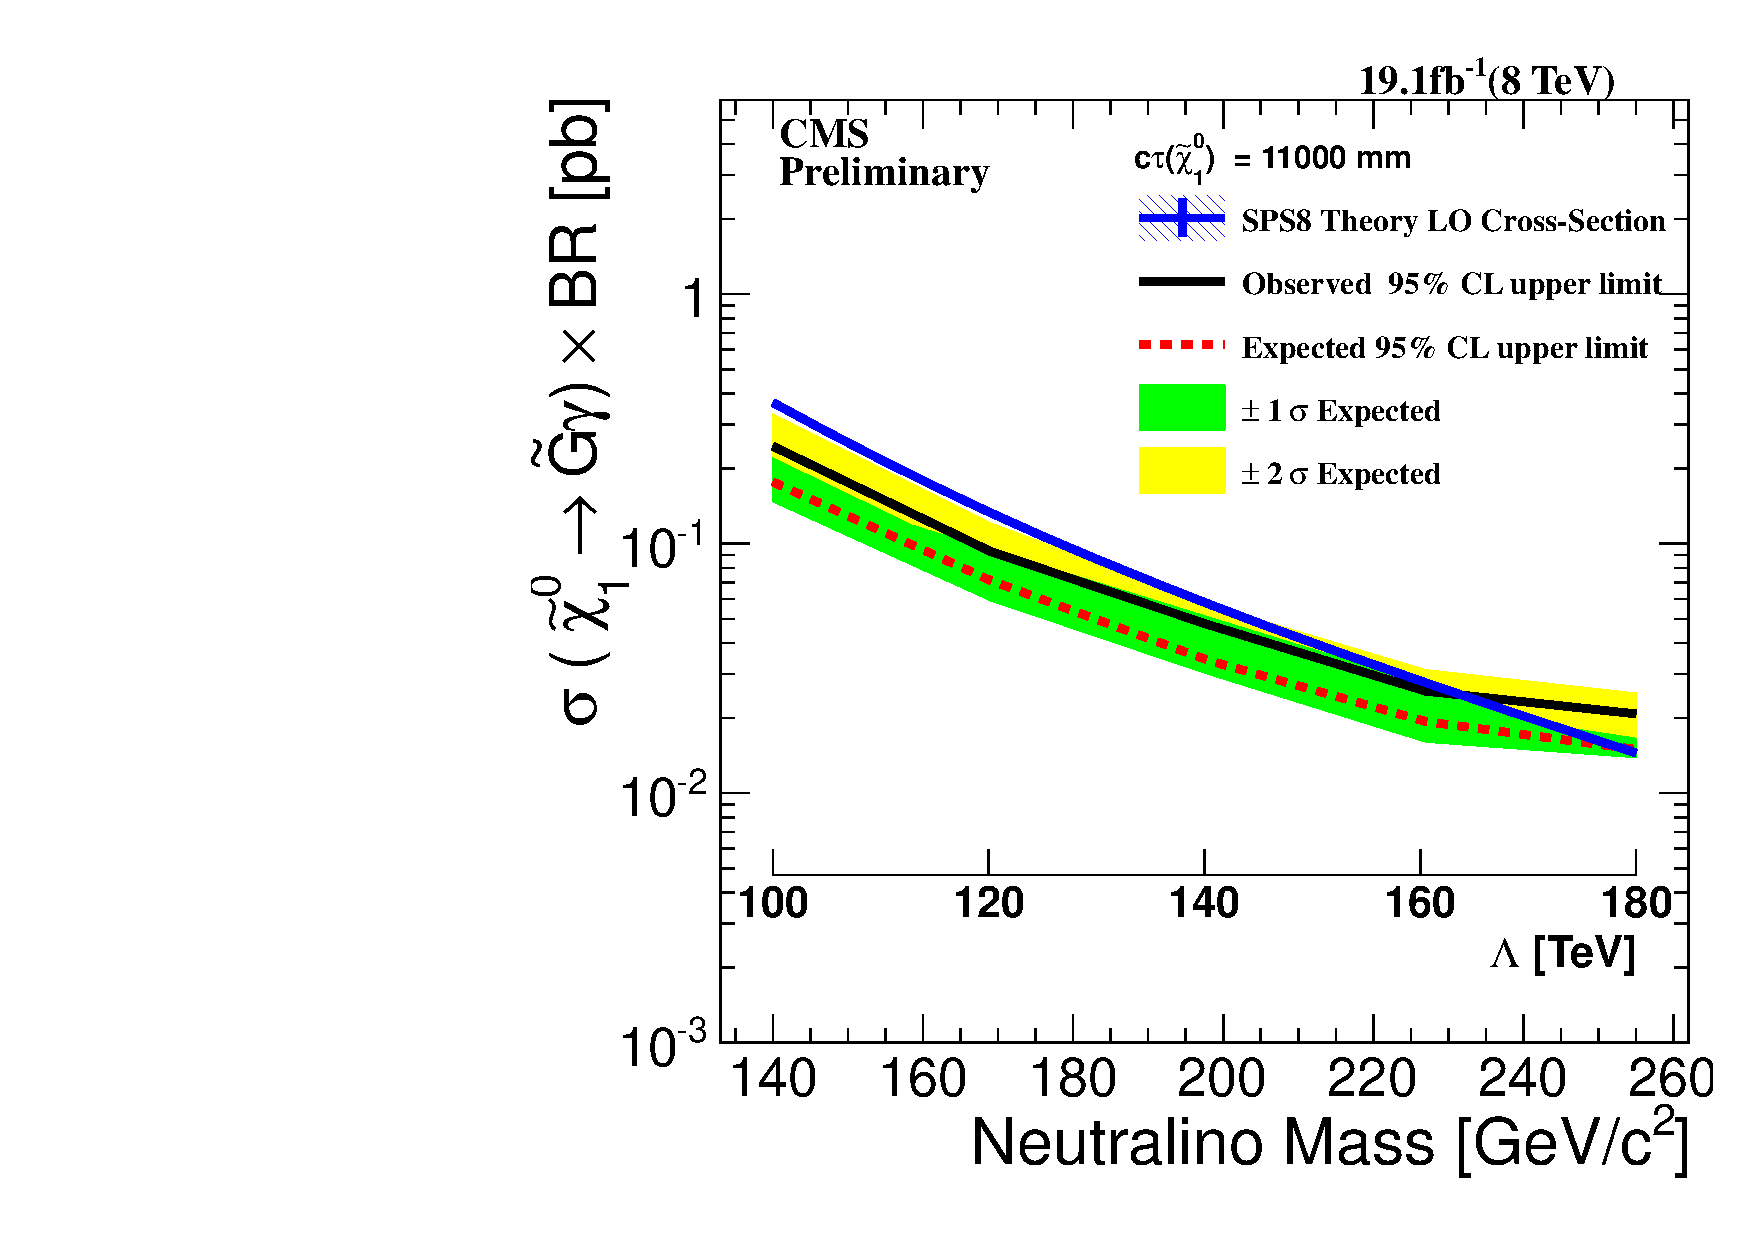
\includegraphics[height=0.8\textwidth, width=0.85\textwidth]{THESISPLOTS/Neutralino_CrosSecVsMass_Exclusion_limit_11000.pdf}
%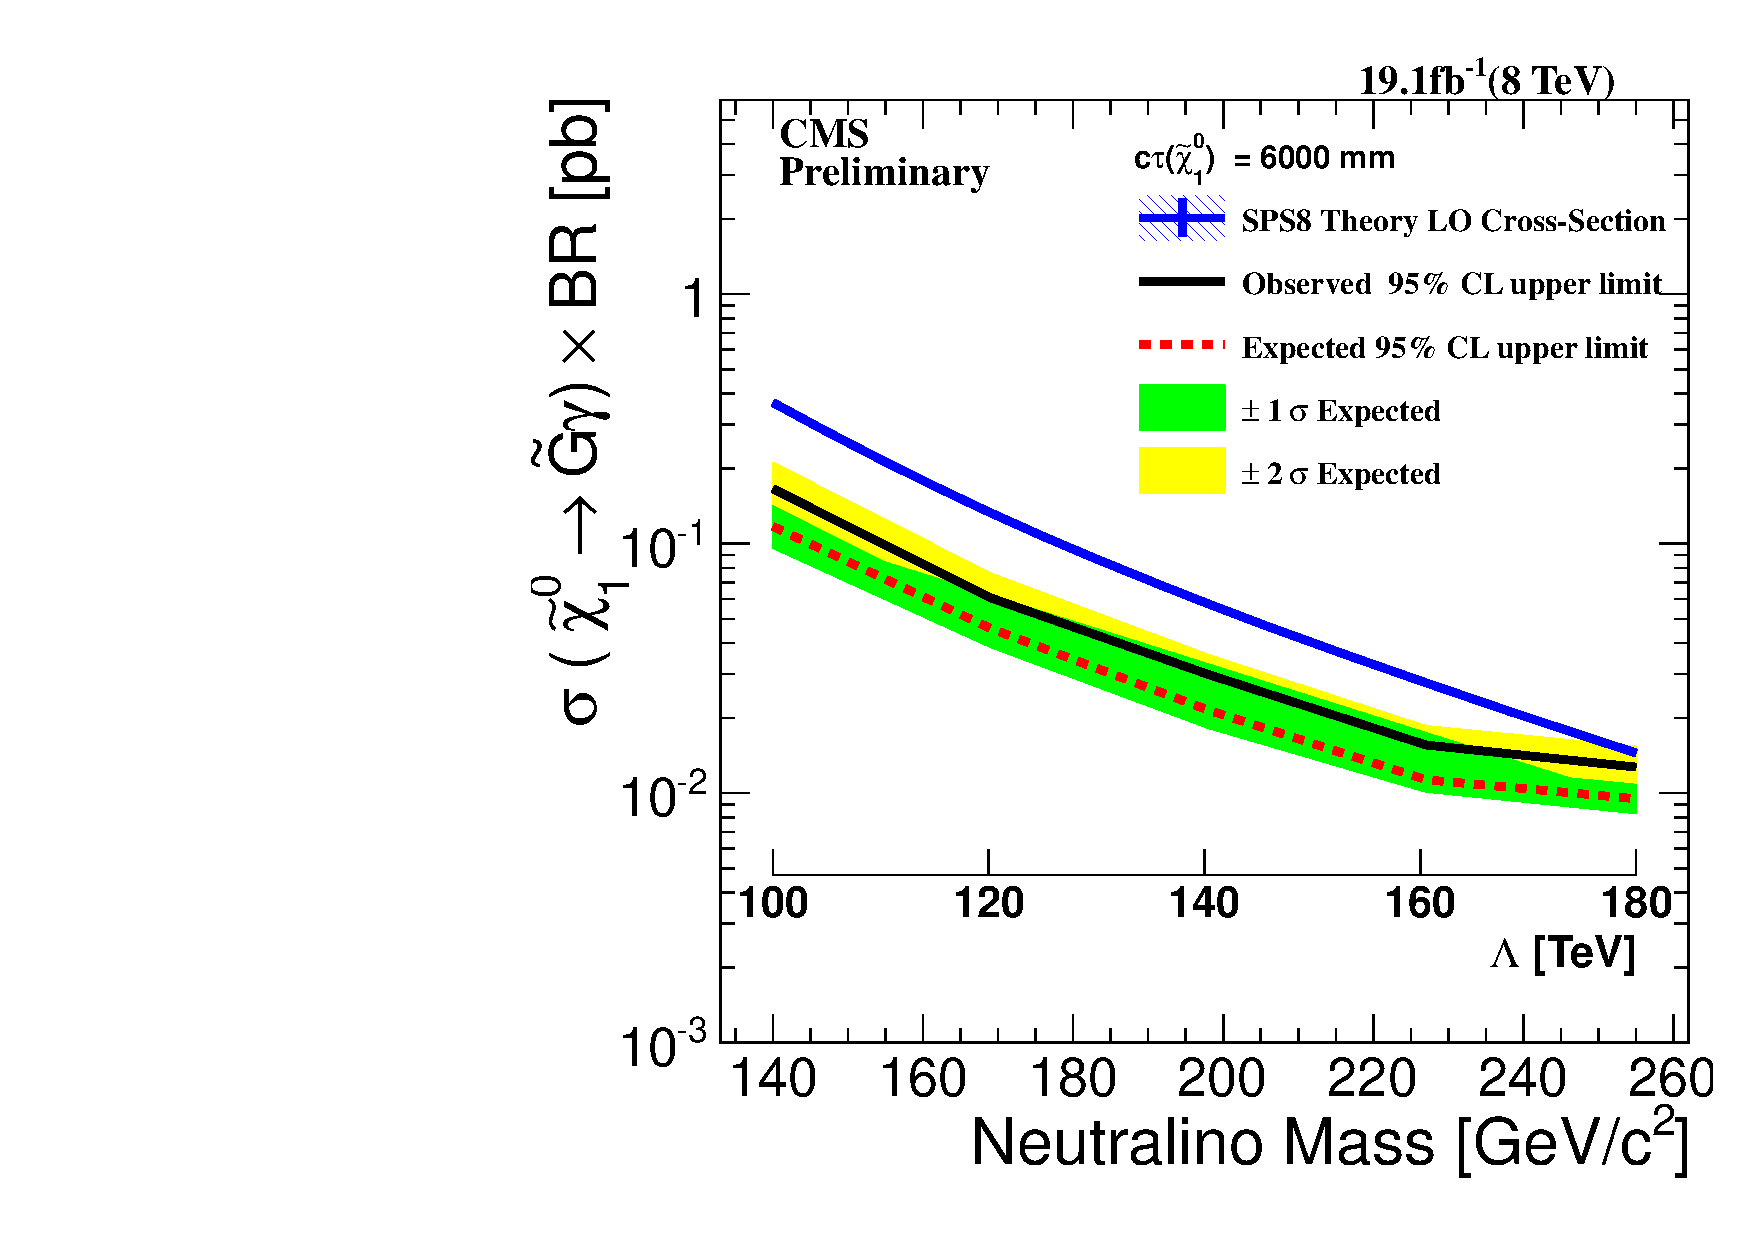
\includegraphics[height=0.65\textwidth, width=0.53\textwidth]{THESISPLOTS/Neutralino_CrosSecVsMass_Exclusion_limit_6000.pdf} }
\captionof{figure}{95\% $CL_{S}$ CL on the lightest neutralino production cross-section times branching ratio~($\sigma\times BR$) for different $\mathbf{\Lambda}$~(or mass of lightest neutralino) for $c\tau = 11000\mm$ or $\tau = 36.7$\ns in the SPS8 benchmark GMSB model.}
\label{fig:MASS-limits}
\end{center}
%\end{figure}
\end{minipage}
\vspace{5mm}

\begin{minipage}{0.95\linewidth}
\begin{center}
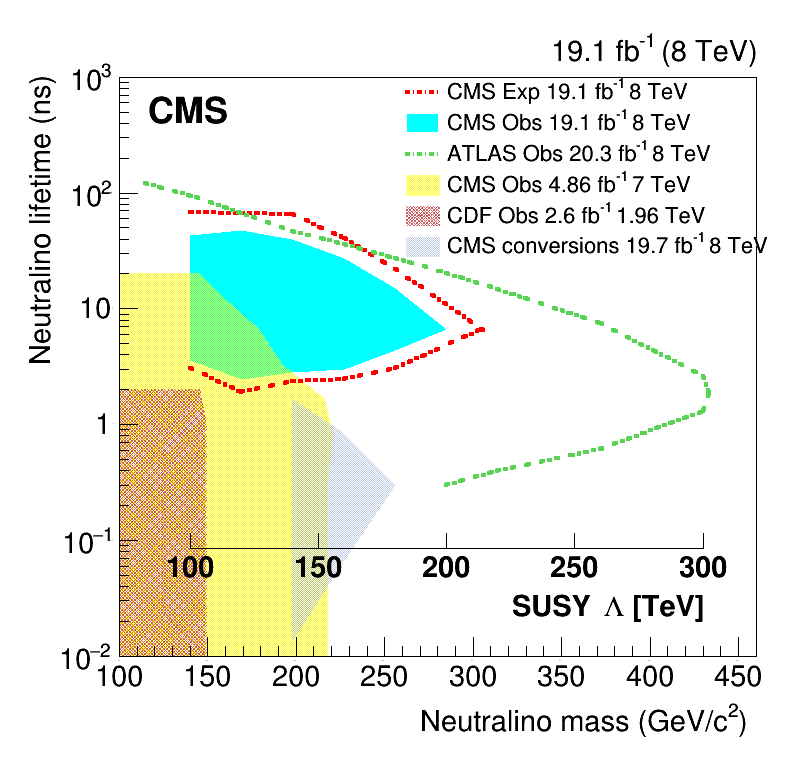
\includegraphics[height=0.85\textwidth, width=0.9\textwidth]{THESISPLOTS/Exclude2D_withAtlas_2015.png}
\captionof{figure}{95\% CL exclusion limit in lightest neutralino mass~(or $\mathbf{\Lambda}$) against mean lifetime in SPS8 benchmark GMSB model. Limits from previous experiments also shown.}
\label{fig:SPS8_2D-Ulimit}
\end{center}
\end{minipage}
\vspace{5mm}

\begin{minipage}{0.95\linewidth}
\begin{center}
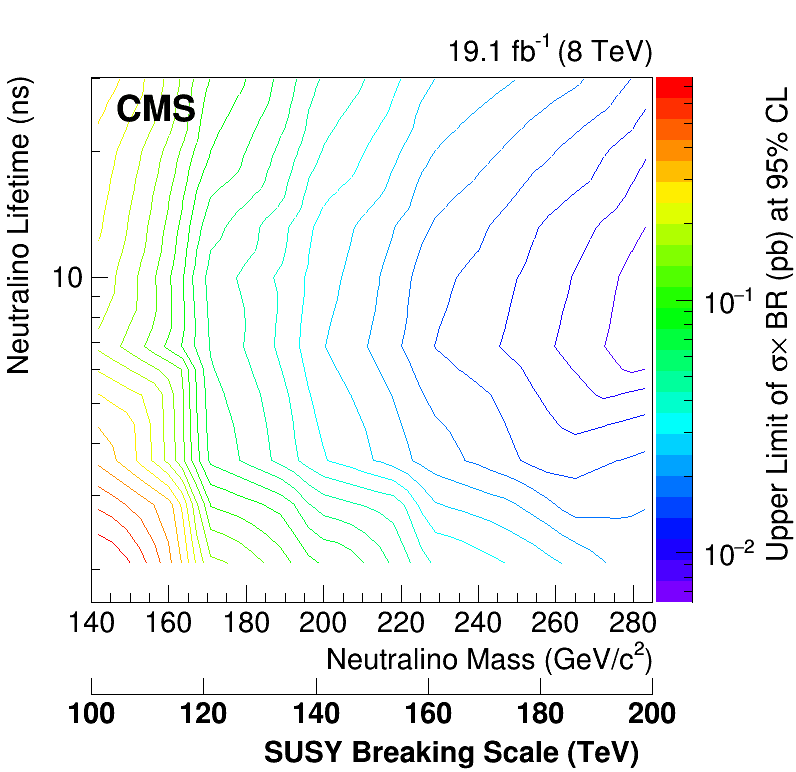
\includegraphics[height=0.85\textwidth, width=0.9\textwidth]{THESISPLOTS/limit2D_Cross-Section-Observed.png}
\captionof{figure}{95\% $CL_{S}$ CL on the cross-section for different mass and lifetime of the lightest neutralino using the 8\TeV data corresponding to an integrated luminosity of 19.1\fbinv of the CMS experiment.}
\label{fig:SPS8_SIGMA-Ulimit}
\end{center}
\end{minipage}
%%\end{landscape}
%% \clearpage% Flush page
%%}

%%%%%%%%%%%%%%%%%%%%%%%%%%%%%%%%%%%%%%%%%%%%%%%%%%%%%%%%%%%%%%%%%%%%%%%%%%%%%%%%%%%%%%%%%%%%%%%%%%%%%%%
%%%%%%%%%%%%%%%%%%%%%%%%%%%%%%%%%%%%%%%%%%%%%%%%%%%%%%%%%%%%%%%%%%%%%%%%%%%%%%%%%%%%%%%%%%%%%%%%%%%%%%%
\begin{comment}
%%is given in table \ref{tab:SIGNALRES}
%%\vspace{5mm}
%%\begin{minipage}{\linewidth} 
%%\begin{center}
%\begin{table}[ht]
%\renewcommand\arraystretch{1.2}
%%\begin{tabular}{c c}
%%\toprule
%%\hline
%%\bfseries{SPS8 GMSB Signal} & \bfseries {Number of Events}\\
%%\hline
%%\toprule
%%\texttt{GMSB(SPS8)}~($\Lambda=180$~TeV,$c\tau=250$~mm) & $0.2096$ \\
%%\texttt{GMSB(SPS8)}~($\Lambda=180$~TeV,$c\tau=500$~mm) & $4.5423$  \\
%%\texttt{GMSB(SPS8)}~($\Lambda=180$~TeV,$c\tau=1000$~mm) & $6.3646$ \\
%%\texttt{GMSB(SPS8)}~($\Lambda=180$~TeV,$c\tau=2000$~mm) & $6.3968$ \\ 
%%\texttt{GMSB(SPS8)}~($\Lambda=180$~TeV,$c\tau=4000$~mm) & $6.1442$ \\
%%\texttt{GMSB(SPS8)}~($\Lambda=180$~TeV,$c\tau=6000$~mm) & $4.6498$ \\
%%\texttt{GMSB(SPS8)}~($\Lambda=180$~TeV,$c\tau=12000$~mm) & $2.918$ \\
%%\hline 
%%\bottomrule
%%\end{tabular}
%%\captionof{table}{Final number for $\Lambda = 180$\TeV GMSB SPS8 MC signal events  events passing our selection cuts.}
%%\label{tab:SIGNALRES}
%\end{table}
%%\end{center}
%%\end{minipage}
\end{comment}

%%%%%%%%%%%%%%%%%%%%%%%%%%%%%%%%%%%%%%%%%%%%%%%%%%%%%%%
%%%%%%%%%%%%%%%%%%%%%%%%%%%%%%%%%%%%%%%%%%%%%%%%%%%%%%%%%%%%%%%%%%%%%%%%%%%%%%%%
% Possible Future Analysis work!
%%%%%%%%%%%%%%%%%%%%%%%%%%%%%%%%%%%%%%%%%%%%%%%%%%%%%%%%%%%%%%%%%%%%%%%%%%%%%%%%
%\section{Future Improvements}
%%%%%%%%%%%%%%%%%%%%%%%%%%%%%%%%%%%%%%%%%%%%%%%%%%%%%%%%%%%%%%%%%%%%

%%%%%%%%%%%%%%%%%%%%%%%%
%%%%%%%%%%%%%%%%%%%%%%%%%%%%%%%%%%%%%%%%%%%%%%%%%%%%%%%%%%%%%%%%%%%%%%%%%%%%%%%%%%%%%%%%%%%%%%%%%%%%%%%%
\begin{comment}
%%In addition to the $p$-value which is used for quantifying the level of incompatibility between the data and a given hypothesis, the HiggsCombine tool also provides a quantity known as the \textit{significance}~($\mathcal{Z}$). $\mathcal{Z}$ and the $p$-value have a very non-linear relation which can be defined using a two-sided fluctuation if a Gaussian variable $\sigma$, with $5\sigma$ significance corresponding to a $p$-value of $p = 5.7 \times 10^{-7}$ to denote a discovery. Since, we have not observed any significant excess of events over our standard model background, we will not mention a lot about significance in this thesis, but rather talk about $p$-values as they are indispensable in computing limits.
%In summary, our hypothesis test is performed using a given statistical method on each value of a chosen parameter of interest~(POI)(usually denoted $\mu$). The $p$-value is obtained from the sampling distribution of the test-statistics being used. Can either obtain this test-statistics analytically or through Monte Carlo computation and  numerical integration. By plotting the $p$-value as a function of the POI, we obtain a $p$-value curve~(in this case the $CL_{s} = \frac{CL_{s+b}}{CL_{b}}$).
%The value of $\mu$ which has a p-value $\alpha = 0.05$ is the upper limit~(for 1-dimensional limits, 2-dimensional limits gives lower and upper limits) of $1 - \alpha$  confidence interval~(\ie 95\%).
%\vspace{5mm}
%\begin{minipage}{0.94\textwidth} 
%\begin{center}
%\mbox{
%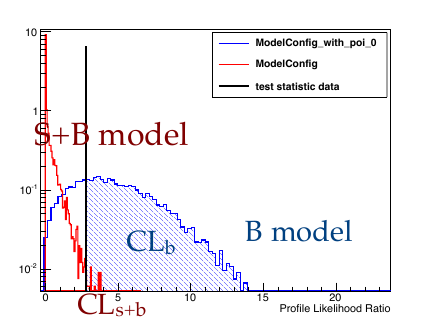
\includegraphics[height=0.65\textwidth, width=0.45\textwidth]{THESISPLOTS/Asymptotics_Test_Stats.png}
%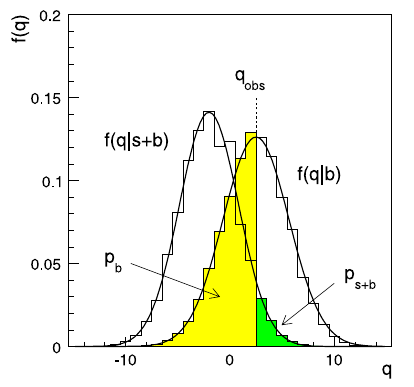
\includegraphics[height=0.615\textwidth, width=0.45\textwidth]{THESISPLOTS/TEST_STATISTICS.png}
%}
%\captionof{figure}{Sampling distributions for $f(t_{\mu}|\mu)$ showing how one extracts the $p$-vlaues. left: is the using a analytic of the Asymptotic method and right: is from the HybridNew method.}
%\label{fig:LIM}
%\end{center}
%\end{minipage}
%\vspace{5mm}
%The important question is always, how does one obtain an expression or a distribution of the test %statistics and $f(t_{\mu}|\mu)$ from the likelihood function? To answer this question, the HiggsCombine tool was developed which consist of various ways of both analytically~(\eg the Asymptotic statistical method \cite{ASYMP}) or through numerical integration or Monte Carlo computation~(\eg the HybridNew statistical method) obtain the test-statistics and $ f(t_{\mu}|\mu)$. We have shown the limit computation results of both methods as used in this analysis.
%As an example, the pdf $ f(t_{\mu}|\mu)$ of the test-statistics~($t_{\mu}$) obtained though the \textcolor{green}{Asymptotic} statistical method as given in \cite{ASYMP} is:
%\begin{equation}\label{eq:ASYPTOTIC}
%f(t_{\mu}|{\mu}^{\prime}) = \mathbf{\Phi}\left( \frac{\mu -{\mu}^{\prime}}{\sigma}\right)\delta(t_{\mu}) +
 %                            \frac{1}{2}\frac{1}{\sqrt{2\pi}}\frac{1}{t_{\mu}}\exp\left[-\frac{1}{2} %\left(  \sqrt{t_{\mu}} - \frac{\mu - {\mu}^{\prime}}{\sigma}\right)^{2} \right]
%\end{equation}
%where result to a half-chi-square distribution when $\mu = \mu^{\prime}$.

%In subtle point worth mentioning is that in the HybridNew approach, systematics uncertainties are taken into account through the Beyesian prior density $\mathbf{\pi(\theta)}$, and the distribution of the test-statistics is computed under the assumption if the Beyesian model of average given as: $$\displaystyle{f(t) = \int f(t|\theta)\pi(\theta)d\theta}$$ and the prior pdf $\mathbf{\pi(\theta)}$ is obtained from some measurements characterized by a given likelihood function $\mathcal{L}_{\mathbf{\theta}}(\mathbf{\theta} )$ which is then used to find the prior using Bayes' Theorem. Unlike other cases where systematic uncertainties are taking as being part of the data and incorporated directly through $\mathcal{G}(\theta)$ as shown in equation \ref{eq:LL}. Nevertheless, they arrive at the same result.
%%%%%%%%%%%%%%%%%%%%%%%%%%%%%%%%%%%%%%%%%%%%%%%%%%%%%%%%%%%%%%%%%%%%%%%%%%%%%% 
%%The accepted method by CMS statistics committee for computing upper upper limit by any search and discovery experiment like ours is to use a profilelikelihood ratio as the test-statistics and a mixture of frequentist-hybrid significance test for the test-statistics calculator and limit extraction. This method is known as the \textit{HybridNew}  method. The parameters of interests~(POI) in our case are the cross-section of signal process and the \textit{nuissance parameters} which are the systematics for the background plus signal model. The sensitivity of the search experiment depends on the systematics and hence the nuissance parameters.
%%%%%%%%%%%%%%%%%%%%%%%%%%
%In a shape based experiment, the mean number of entries in the $i$th bin of the histogram from signal and background will be given as 
%\begin{equation}
%s_{i} = s_{tot} \int_{bin, i} f_{s}\left(t;\mathbf{\theta_{s}}\right) ,\quad 
%b_{i} = b_{tot} \int_{bin, i} f_{b}\left(t;\mathbf{\theta_{b}}\right)
%\end{equation}
%where the functions $f_{s}\left(t;\mathbf{\theta_{s}}\right) $ and $f_{b}\left(t;\mathbf{\theta_{b}}\right) $ are the probability density functions~(Pdfs) of the variable $t$~(ECAL time) for the signal and background events, respectively, and $\mathbf{\theta_{s}} $ and $\mathbf{\theta_{b}} $ represent the parameters which characterize the shapes of the Pdfs. $s_{tot}$ and $b_{tot}$ represents the total mean number of signal and background events, respectively, while each integral gives the probability for an event to be found in bin $i$. $\mathbf{\theta} = \left( \mathbf{\theta_{s}}, \mathbf{\theta_{b}}, b_{tot} \right)$ denote all nuisance parameters~(systematic uncertainties) and $s_{tot}$ is the signal normalization which is fixed to the value predicted by the nominal signal model.

%The $CL_{s}$ method advantage in search experiments where  . The method is used for making statistical inferences by computing the probability or \textit{p-value} from  \textit{test-statistics} of the different hypothesis to be tested. From these $p$-values the CL is computed and the exclusion limits derived. The computation of the CL from the results of the hypothesis testing is according to the following procedure:
%%\begin{itemize}
%\item A \textit{Null}~($H_{0}$) and an \textit{Alternate}~($H_{1}$) hypothesis are defined. Additional hypothesis can also be defined, however, in our case we have just two hypothesis to test,
%\item A test-statistics~($t(x)$), where $x$ is the data histogram variable, and its corresponding test %statistics calculator are selected,
%\item The confidence limit is computed by inverting the results of the hypothesis test.
%\end{itemize}
%Before we discuss the limit computation, first, let us describe the CLs technique.
%\par 
%%%%%%%%%%%%%%%%%%%%%%%%%%%%%%%%%%%%%%%%%%%%%%%%%%%%%%%%%%%%%%%%%%%%%
% The acceptance is because it has been tested and validated during the search for the Higgs boson at a previous CERN experiment known as LEP and recently in the discovery of the Higgs boson with mass, $m_{H} = 125.36\pm 0.37(stat.Unc)\pm0.18(syst.Unc)$, in 2012, by both CMS and ATLAS experiments.
%where $s+b$ means signal plus background, $CL_{s+b}$ or $p_{s+b}$ is the $p$-value of the signal plus background hypothesis and $CL_{b}$ or $p_{b}$ is that for the background only hypothesis.
\end{comment}

\begin{comment}
%The reason for using the $CL_{s}$ method is because in search  and discovery experiments the discrimination between the background-only hypothesis with the signal plus background hypothesis is very poor and there is a huge overlap between the probability density functions~(pdfs) of the test-statistics of both hypothesis as shown in Figure \ref{fig:CLS}, where the magenta-colored function and shaded area under the pdf is for the background-only hypothesis pdf and the blue is for the signal plus background hypothesis pdf. Each area under the corresponding pdf is the probability or $p$-value computed from the observed value of the test-statistics from data, $q^{obs}_{1}$,  to higher values.
%exclusion limit is not easily moved by fluctuations in the background \cite{LIM}. 

%\vspace{5mm}
%\begin{minipage}{0.90\linewidth} 
%\begin{center}
%\mbox{
%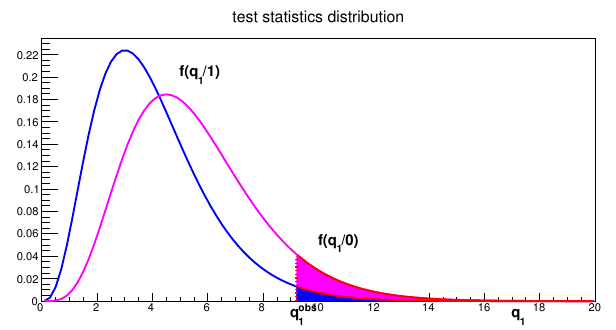
\includegraphics[height=0.55\textwidth, width=0.7\textwidth]{THESISPLOTS/CLS_METHOD.png}}
%\captionof{figure}{Test statistic probability density functions~(pdfs) of the signal plus background hypothesis~(blue) and background-only~(magenta) hypothesis showing a typical scenario where using the $CL_{s}$ approach instead of the $CL_{s+b}$ leads to better or conservative exclusion limits.}
%\label{fig:CLS}
%\end{center}
%\end{minipage}
\end{comment}
%%%%%%%%%%%%%%%%%%%%%%%%%%%%%%%%%%%%%%%%%%%%%%%%%%%%%%%%%%%%%%%%%%%%%%%%%%%%%%%%%%%%%%%%%%%%%%%%%%%%
%%%%%%%%%%%%%%%%%%%%%%%%%%%%%%%%%%%%%%%%%%%%%%%%%%%%%%%%%%%%%%%%%
%We also produce a two dimensional limit in $\tau_{\PSneutralinoOne}$ and $m_{\PSneutralinoOne}$~(\GeVcc) still using the CLs technique.
%\newline
%Using  the upper limits in $\tau$ and mass of the lightest neutralino or effective SUSY breaking scale, $\mathbf{\Lambda}$, we produce a two dimensional exclusion limit in $\tau$ and $\mathbf{\Lambda}$ and also a cross-section limit according to the SPS8 benchmark GMSB model. 

%%\vspace{5mm}
%%\begin{minipage}{0.94\textwidth} 
%%\begin{center}
%\mbox{
%%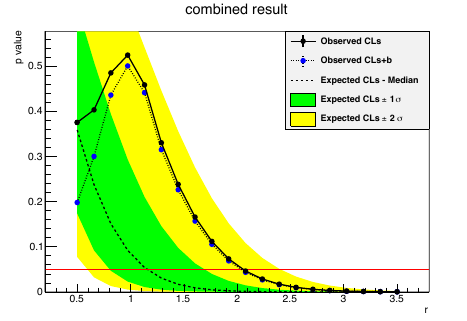
\includegraphics[height=0.45\textwidth, width=0.55\textwidth]{THESISPLOTS/Limits_CLs.png}
%%\captionof{figure}{Distribution of $p$-vlaues showing how upper limit on $\mu$ is extracted for a given threshold probability.}
%%\label{fig:LIMITS_CLS}
%%\end{center}
%%\end{minipage}

